\section{Data}
\label{sec:data}
De evolutie die het design in deze iteratie heeft ondervonden is vooral te merken in de database.
Het datamodel is uitgebreid opdat de databank in staat is om vakken, lokalen en allerhande concepten omtrend deze vakken en lokalen op te kunnen slaan. Deze concepten zullen laterinvloed hebben op het plannen van de lessenroosters en lokalenroosters via de scheduler.\\

Ook werden aanpassingen uitgevoerd aan het user management zodat bij implementatie gebruik gemaakt kon worden van de module Spring Security\cite{spring-security} om de authenticatie van gebruikers af te handelen.\\

Figuur~\ref{fig:EER diagram} toont het EER-model van de databank. Om overzicht te bewaren worden de attributen die iedere entiteit bezit niet weergegeven in dit model.

\begin{figure}[H]
	\centering
	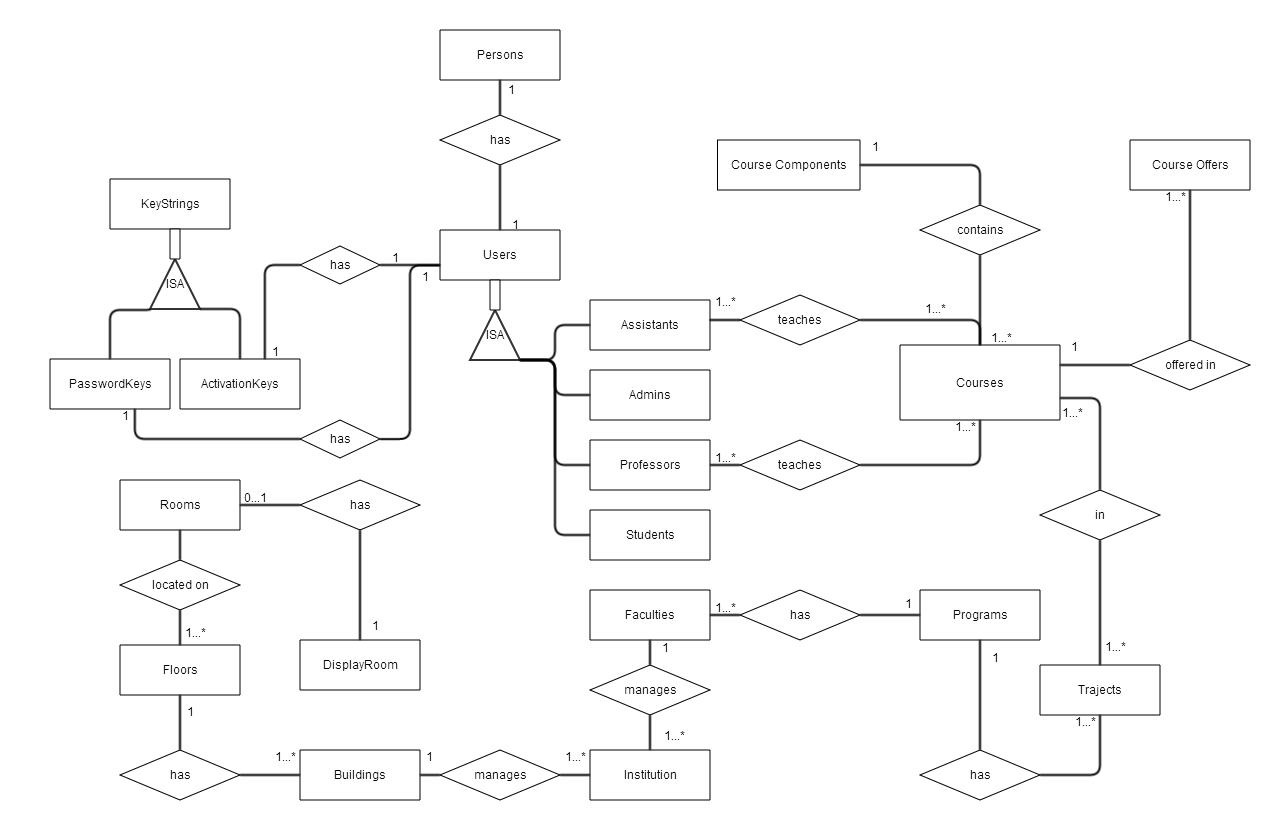
\includegraphics[scale=0.4]{img/ER2-gliffy}
	\caption{EER diagram}
	\label{fig:EER diagram}
\end{figure}
